\section{Friction model}

The effort measured on the sbRIO is equal to the sum of the force required to overcome friction and the external forces applied to the end-effector. For the system to be transparent, the force required to overcome friction should not be fed back as this force would not be felt if the teleoperator was holding the tool directly. In order to isolate the external forces a friction model is required. The model built is based on the one derived in \cite{force_reflection} that describe the friction in a motor. However in the model it was decided to consider the motor and the EndoWrist as one element as no dynamic model for the motor alone is derived. Thus, the model estimates the sum of the friction in the EndoWrist and in the motor.
The total friction acting on the actuator can be written as:

\begin{equation}
\tau_f = \tau_v + \tau_c + \tau_s
\label{eq:total_friction}
\end{equation} 

with:\\
\hspace*{8mm} $\tau_v$ viscous friction\\
\hspace*{8mm} $\tau_c$ coulomb friction\\
\hspace*{8mm} $\tau_s$ static friction    


The viscous friction is proportional to the opposite of the velocity:
\begin{equation}
\tau_v = F * w;
\label{eq:viscous_friction}
\end{equation}
with:\\
\hspace*{8mm}$w$ the angular velocity\\
\hspace*{8mm}$F$ a negative coefficient\\

The coefficient $F$ can be computed from the measurements made on the setup by plotting the effort depending on the velocity.

The stiction is the amount of effort required for the object to start moving when its velocity is zero. As such it can be described as:

\begin{equation} 
\tau_s =  \begin{cases} K_s, & \mbox{if } w = 0 \\ 0, & \mbox{else} \end{cases}
\label{eq:static_friction}
\end{equation}
with:\\
\hspace*{8mm}$w$ the angular velocity\\
\hspace*{8mm}$K_s$ a constant\\

The constant $K_s$ can be measured by increasing the current supplied to the motor until it starts moving. 
The coulomb friction occurs as a constant force opposing the movement:

\begin{equation}
\tau_c = sign(w)*K_c;
\label{eq:coulomb_friction}
\end{equation}
with:\\
\hspace*{8mm}$w$ the angular velocity\\
\hspace*{8mm}$K_c$ a constant determined experimentally\\
\hspace*{8mm}the $sign$ function is defined as $sign(w) = \begin{cases} 1, & \mbox{if } w > 0 \\ 0, & \mbox{if } w == 0 \\ -1, & \mbox{if } w < 0\end{cases}$\\

The constant $K_c$ can be measured by setting the motor in motion and decreasing the current until the motor stops moving.
From \eqref{eq:viscous_friction} to \eqref{eq:coulomb_friction}, the total friction given by \eqref{eq:total_friction} can be plotted as:

\begin{figure}[h]
\centering
	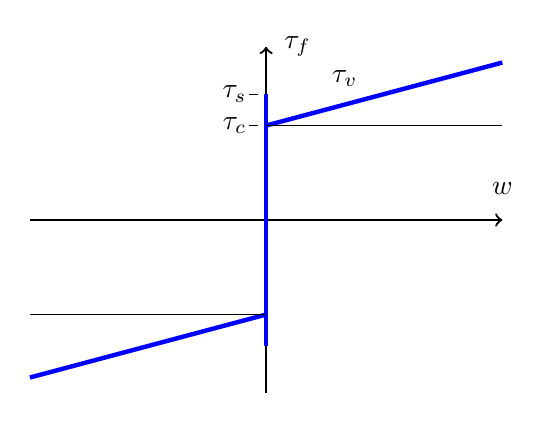
\begin{tikzpicture}
	\draw [->,thick] (-3,0) -- (3,0);
	\draw [->,thick] (0,-2.2) -- (0,2.2);
	\draw [ultra thick, color=blue] (0,-1.6) -- (0,1.6);
	\draw [ultra thick, color=blue] (0,1.2) -- (3,2);
	\draw [ultra thick, color=blue] (0,-1.2) -- (-3,-2);
	\draw (0,1.2) -- (3,1.2);
	\draw (0,-1.2) -- (-3,-1.2);

	\node at (-0.4,1.6) {$\tau_s$};
	\draw (-0.22,1.6) -- (-0.1,1.6);
	\node at (-0.4,1.2) {$\tau_c$};
	\draw (-0.22,1.2) -- (-0.1,1.2);
	\node at (1,1.8) {$\tau_v$};


	\node at (3,0.4) {$w$};
	\node at (0.4,2.2) {$\tau_f$};

	\end{tikzpicture}
\caption{friction}
\end{figure}


\todo{add estimation of the 3 parameters that justify that we don't need viscous / static}